
\subsubsection{ProcessorEngine}
Le simulateur doit offrir une certaine modularité afin de permettre d'apprécier l'incidence des choix de conception sur le code assembleur et sur l'exécution. 

Les propriétés du processeur sont gérées par la classe \pyinline{ProcessorEngine}

On pourra donc définir le modèle de processeur retenu à l'aide d'un dictionnaire qui prend pour clés:
\begin{itemize}
	\item le nom du modèle associé: \pyinline{'name': str};
	\item la taille des registres: \pyinline{'register_bits': int};
	\item la taille des mots: \pyinline{'data_bits': int};
	\item la capacité ou non de réorienter la sortie de l'UAL vers un registre quelconque: \pyinline{'free_ual_output':bool}. Si \pyinline{False}, la sortie de l'UAL sera systématique le registre 0. Il convient alors de libérer celui-ci; 
	\item la liste des commandes pouvant accepter directement des littéraux \pyinline{'litteralCommands':Dict[str,Commands]};
	\item la liste des commandes admissibles \pyinline{'commands':Dict[str,Commands]}.
\end{itemize}

Chaque \pyinline{Command} correspond à un dictionnaire qui prends pour clés:
\begin{itemize}
	\item un code binaire \pyinline{'opcode': str,}. Le choix des \pyinline{opcode} est fait de telle sorte que la taille des mots soit op
	\item une commande assembleur \pyinline{'asm': str},
	\item la taille du littéral associé	\pyinline{'litteral_bits': int}
\end{itemize}

Deux modèles sont implémentés par défaut dans le simulateur.

\begin{minipage}[t]{0.48\textwidth}
	\captionof{table}{Processeur 16 bits}
\begin{minipage}[t]{0.5\textwidth}
	\vspace{0cm}
	\centering
		\begin{tabular}{l|>{\ttfamily\footnotesize}l}
		\pyinline{register_bits}&	3\\ \hline
		\pyinline{free_ual_output}&	True
\\\hline
		\pyinline{data_bits}&	16\\
		\end{tabular}
	
	\vspace{1cm}
	
	\begin{tabular}{>{\ttfamily\footnotesize}c|>{\ttfamily\footnotesize}c|>{\ttfamily\footnotesize}c}
		\multicolumn{3}{c}{\pyinline{litteralCommands}}\\\hline\hline
		Nom	& OPCODE & ASM\\\hline
		neg                & 010110 & NEG  \\
		move               & 01001  & MOVE \\
		+                  & 1000  & ADD  \\
		-                  & 1001  & SUB  \\
		*                  & 1010  & MULT \\
		/                  & 1011  & DIV  \\
		\%                 & 1100  & MOD  \\
		\&                 & 1101  & AND  \\
		|                  & 1110  & OR   \\
		\textasciicircum{} & 1111  & XOR  \\
		$\sim$             & 010111 & NOT 
	\end{tabular}
\end{minipage}
\begin{minipage}[t]{0.5\textwidth}
	\vspace{0cm}	
	\centering
		\begin{tabular}{>{\ttfamily\footnotesize}c|>{\ttfamily\footnotesize}c|>{\ttfamily\footnotesize}c}
		\multicolumn{3}{c}{\pyinline{Commands}}\\\hline\hline
		Nom	& OPCODE & ASM\\\hline
halt               & 00000      & HALT  \\
goto               & 000001      & JMP   \\
!=                 & 0001000   & BNE   \\
==                 & 0001001   & BEQ   \\
\textless{}        & 0001010   & BLT   \\
\textgreater{}     & 0001011   & BGT   \\
cmp                & 00011     & CMP   \\
print              & 00100    & PRINT \\
input              & 00101    & INPUT \\
load               & 0011     & LOAD  \\
move               & 01000   & MOVE  \\
neg                & 010100  & NEG   \\
$\sim$             & 010101  & NOT   \\
+                  & 0110000 & ADD   \\
-                  & 0110001 & SUB   \\
*                  & 0110010 & MULT  \\
/                  & 0110011 & DIV   \\
\%                 & 0110100 & MOD   \\
\&                 & 0110101 & AND   \\
|                  & 0110110 & OR    \\
\textasciicircum{} & 0110111 & XOR   \\
store              & 0111    & STORE
\end{tabular}
\end{minipage}
\end{minipage}
\hfill
\begin{minipage}[t]{0.48\textwidth}
	\captionof{table}{Processeur 12 bits}
	\begin{minipage}[t]{0.5\textwidth}
		\vspace{0cm}
		\centering
		\begin{tabular}{l|>{\ttfamily\footnotesize}l}
			\pyinline{register_bits}&	2\\ \hline
			\pyinline{free_ual_output}&	False
\\\hline
			\pyinline{data_bits}&	12\\
		\end{tabular}
		
		\vspace{1cm}
		
		\begin{tabular}{>{\ttfamily\footnotesize}c|>{\ttfamily\footnotesize}c|>{\ttfamily\footnotesize}c}
			\multicolumn{3}{c}{\pyinline{litteralCommands}}\\\hline\hline
			Nom	& OPCODE & ASM\\\hline
			\multicolumn{3}{c}{\pyinline{NONE}}\\\hline\hline
		\end{tabular}
	\end{minipage}
	\begin{minipage}[t]{0.5\textwidth}
		\vspace{0cm}
		\centering
		\begin{tabular}{>{\ttfamily\footnotesize}c|>{\ttfamily\footnotesize}c|>{\ttfamily\footnotesize}c}
			\multicolumn{3}{c}{\pyinline{Commands}}\\\hline\hline
			Nom	& OPCODE & ASM\\\hline
			halt               & 0000       & HALT  \\
			goto               & 0001        & JMP   \\
			==                 & 0010       & BEQ   \\
			\textless{}        & 0011       & BLT   \\
			cmp                & 11110101 & CMP   \\
			print              & 0100      & PRINT \\
			input              & 0101      & INPUT \\
			load               & 100      & LOAD  \\
			move               & 11110110 & MOVE  \\
			$\sim$             & 11110111 & NOT   \\
			+                  & 11111000 & ADD   \\
			-                  & 11111001 & SUB   \\
			*                  & 11111010 & MULT  \\
			/                  & 11111011 & DIV   \\
			\%                 & 11111100 & MOD   \\
			\&                 & 11111101 & AND   \\
			|                  & 11111110 & OR    \\
			\textasciicircum{} & 11111111 & XOR   \\
			store              & 101      & STORE
		\end{tabular}
	\end{minipage}
\end{minipage}

La classe \pyinline{ProcessorEngine} a la responsabilité entre autre d'assurer que le modèle de processeur soit consistant, d'assurer la conversion entre code assembleur et code binaire.
\begin{sidewaysfigure}
	\centering
		
\tikzset{
	every leaf node/.style={draw=black, rectangle, align=center},
	every tree node/.style={font=\tiny},
	tt/.style={font=\ttfamily},
}
\forestset{tikzQtree/.style={for tree={l sep=3em, anchor=center, if n children=0{
				node options=every leaf node/.try}{node options=every tree node/.try}}}}
	\scriptsize
	\begin{forest}
		tikzQtree
[	,
	[ 0,
		[ 00,
			[ 000, 
				[ 0000
					[00000[\texttt{HALT}]],[00001[\texttt{JUMP}]]
				],
				[ 0001,
					[ 00010,
						[ 000100,
							[0001000[\texttt{BNE}]], [0001001[\texttt{BEQ}]]
						],
						[ 000100,
							[0001010[\texttt{BLT}]], [0001011[\texttt{BGT}]]
						]
					],
					[00011[\texttt{CMP}]]
				]
			],
			[ 001,
				[ 0010,
					[00100[\texttt{PRINT}]], [00101[\texttt{INPUT}]]
				],
				[0011[\texttt{LOAD}]]
			]
		],
		[ 01,
			[ 010,
				[ 0100,
					[01000[\texttt{MOVE}]], [01001[\texttt{MOVE}]],
				],
				[ 0101,
					[ 01010,
						[010100[\texttt{NEG}]], [010101[\texttt{NOT}]]
					],
					[ 01011,
					[010110[\texttt{NEG}]], [010111[\texttt{NOT}]]
					]
				]
			],
			[011
				[0110,
					[01100,
						[011000,
							[0110000[\texttt{ADD}]], [0110001[\texttt{SUB}]]
						],
						[011001,
							[0110010[\texttt{MULT}]], [0110011[\texttt{DIV}]]
						]
					],
					[01101,
						[011010,
							[0110100[\texttt{MOD}]], [0110101[\texttt{AND}]]
						],
						[011011,
							[0110110[\texttt{OR}]], [0110111[\texttt{XOR}]]
						]
					],
				],
				[0111[\texttt{STORE}]]
			]
		]
	], 
	[1,
		[10,
			[100,
				[1000[\texttt{ADD}]], [1001[\texttt{SUB}]]
			],
			[101,
				[1010[\texttt{MULT}]], [1011[\texttt{DIV}]]
			]
		],
		[11,
			[110,
				[1100[\texttt{MOD}]], [1101[\texttt{AND}]]
			],
			[111,
				[1110[\texttt{OR}]], [1111[\texttt{XOR}]]
			]
		]
	]	
]
\end{forest}
		\caption{Langage 16 bits - OPCODE et ASM}
\end{sidewaysfigure}

\begin{sidewaysfigure}
	\centering
	
\tikzset{
	every leaf node/.style={draw=black, rectangle, align=center},
	every tree node/.style={font=\tiny},
	tt/.style={font=\ttfamily},
}
\forestset{tikzQtree/.style={for tree={l sep=3em, anchor=center, if n children=0{
				node options=every leaf node/.try}{node options=every tree node/.try}}}}
	\scriptsize
	\begin{forest}
		tikzQtree
[	,
	[ 0,
		[00,
			[000,
				[0000[HALT]],
				[0001[JMP]]
			],
			[001,
				[0010[BEQ]],
				[0011[BLT]]
			]
		],
		[01,
			[010,
				[0100[PRINT]],
				[0101[INPUT]]
			]
		]
	], 
	[1,
		[10,
			[100[LOAD]],
			[101[STORE]]
		],
		[11,
			[111,
				[1111,
					[11110,
						[111101,
							[1111010,
								[11110101[CMP]]
							],
							[1111011,
								[11110110[MOVE]],
								[11110111[NOT]]
							]
						]
					],
					[11111,
						[111110,
							[1111100,
								[11111000[ADD]],
								[11111001[SUB]]
							],
							[1111101,
								[11111010[MULT]],
								[11111011[DIV]]
							]
						],
						[111111,
							[1111110,
								[111111100[MOD]],
								[111111101[AND]]
							],
							[1111111,
								[111111110[OR]],
								[111111111[XOR]]
							]
						]
					]
				]
			]
		]
	]	
]
\end{forest}
	\caption{Langage 12 bits - OPCODE et ASM}
\end{sidewaysfigure}

\clearpage
\subsubsection{Executeur}

Lors de l'exécution, le processeur modèle est représenté par un objet de classe \pyinline{Executeur} (figure \ref{fig:class_Executeur}). Les différents paramètres (taille des registres, taille mémoire, fonctionnement UAL) sont définis par la classe \pyinline{ProcessorEngine} associée. Afin de permettre le suivi de l'exécution, l'\pyinline{Executeur} implémente entre autre:
\begin{itemize}
	\item 2 bus de données: \pyinline{_DATA_BUS} et \pyinline{_DATA_BUS_2};
	\item une mémoire: \pyinline{_MEMORY}
	\item un registre adresse mémoire \pyinline{_MEMORY_ADDRESS} et un registre instruction \pyinline{_INSTRUCTION_REGISTER}
	\item un pointeur de ligne \pyinline{_LINE_POINTER}
	\item une sortie affichage \pyinline{_PRINT}
	\item un buffer \pyinline{_BUFFER}
	\item une UAL \pyinline{_UAL}
\end{itemize}



Chaque composant est modélisé par une instance d'une classe dédiée ( \pyinline{ScreenComponent}, \pyinline{UalComponent}, \pyinline{RegisterGroup}, etc...) implémentant les méthodes associées au comportement de chaque composant physique, par exemple pour l'UAL:
\begin{itemize}
	\item définir l'opération à venir: \pyinline{setOperation()};
	\item mémoriser le premier opérande:\pyinline{writeFirstOperand()};
	\item mémoriser le second opérande: \pyinline{writeSecondOperand()};
	\item exécuter le calcul: \pyinline{execCalc()};
	\item lire le résultat: \pyinline{read()};
\end{itemize}


\begin{figure}[h!]
	\centering
	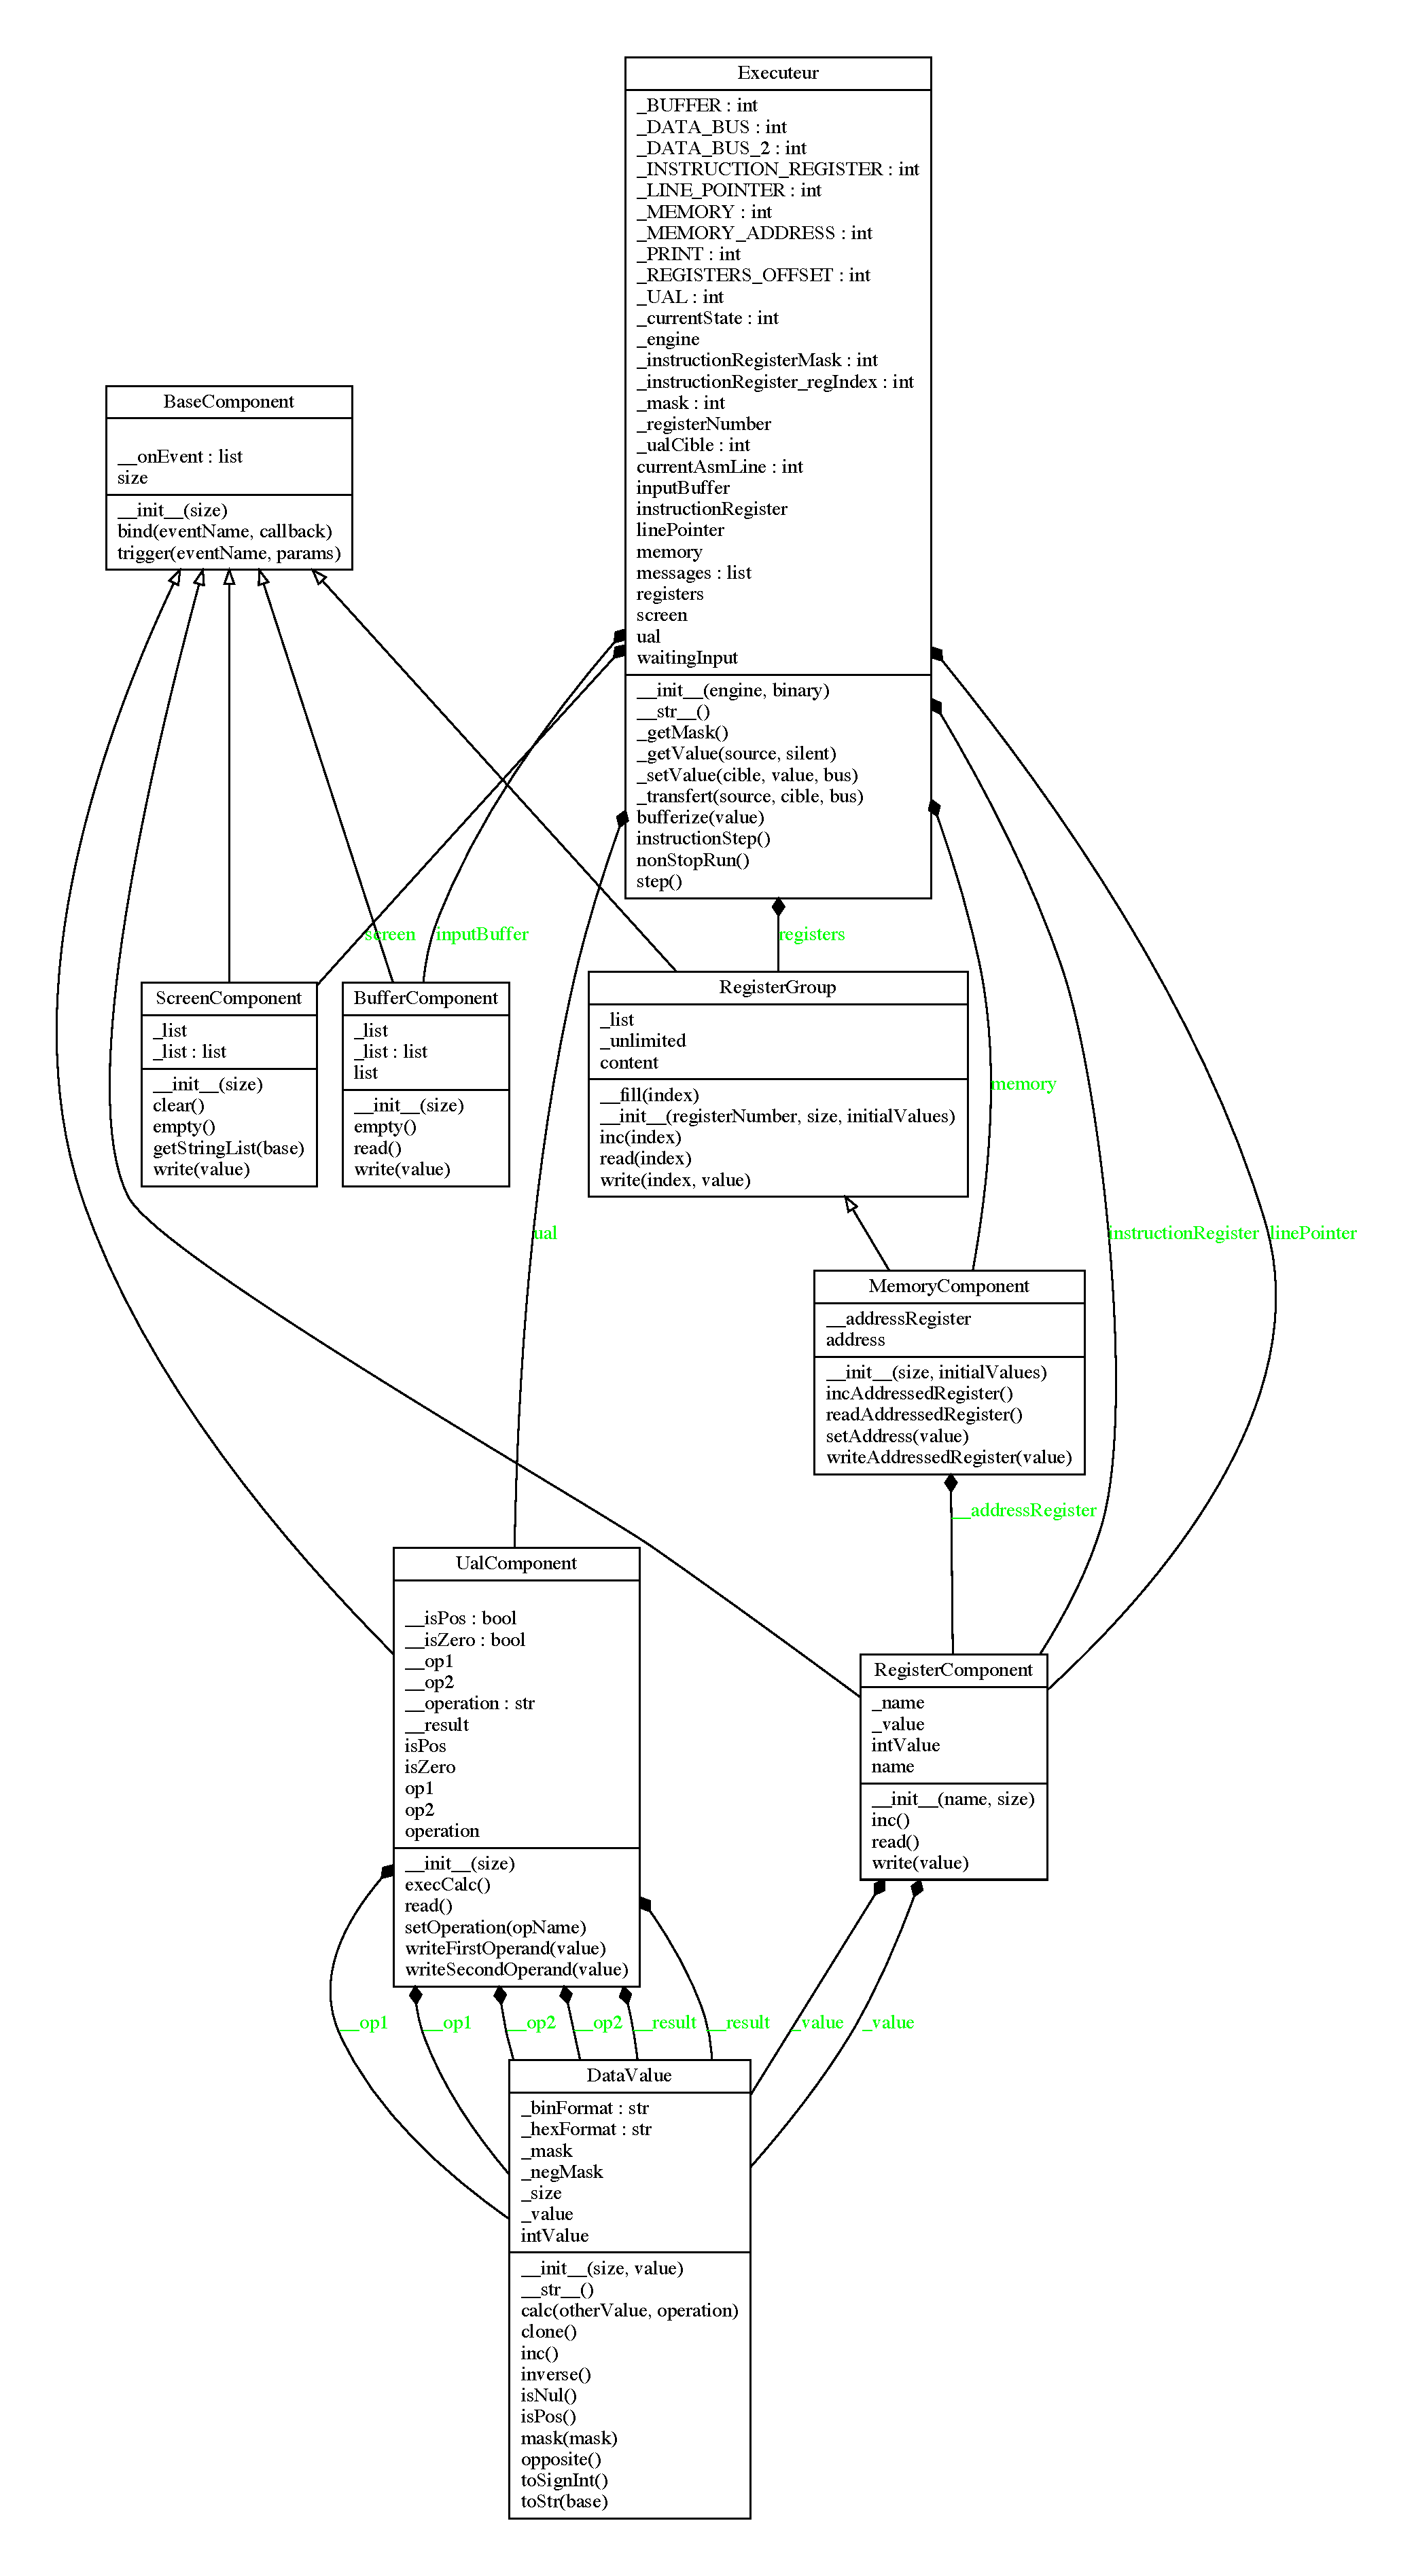
\includegraphics[height = 0.85\textheight]{./Pictures/Executeur.pdf}
	\caption{\label{fig:class_Executeur} Diagramme de classe - Executeur}
\end{figure} 

\clearpage